\documentclass{ieeeaccess}
\usepackage{cite}
\usepackage{amsmath,amssymb,amsfonts}
\usepackage{algorithmic}
\usepackage{algorithm}
\usepackage{graphicx}
\usepackage{textcomp}
\usepackage{booktabs}
\usepackage{float}
\usepackage{wrapfig}
\def\BibTeX{{\rm B\kern-.05em{\sc i\kern-.025em b}\kern-.08em
    T\kern-.1667em\lower.7ex\hbox{E}\kern-.125emX}}
\begin{document}
%%\history{Date of publication xxxx 00, 0000, date of current version xxxx 00, 0000.}%%
%%\doi{10.1109/ACCESS.2024.DOI}%%

\title{Hybrid Knowledge-Graph-Enhanced Retrieval-Augmented Generation for Academic Information Systems}

\author{
\uppercase{Julia Mariam John}\authorrefmark{1},
\uppercase{Nirmel B. Joseph}\authorrefmark{1},
\uppercase{Rohith N.S.}\authorrefmark{1}
}

\address[1]{Department of Computer Science \& Engineering, Mar Baselios College of Engineering and Technology, Thiruvananthapuram, India
(e-mail:juliamariamjohn.b23cs2137@mbcet.ac.in; nirmelbjoseph.b23cs2148@mbcet.ac.in; rohithns.b23cs2156@mbcet.ac.in)}

\tfootnote{This work was conducted at Mar Baselios College of Engineering and Technology, Thiruvananthapuram, India.}

\markboth
{ Hybrid KG-RAG for Academic Information Systems}
{ Hybrid KG-RAG for Academic Information Systems}

%%\corresp{Corresponding author: Julia Mariam John (e-mail: juliamariamjohn.b23cs2137@mbcet.ac.in).}%%

\begin{abstract}
Retrieving precise academic information from institutional websites remains a persistent challenge due to fragmented, unstructured, and multi-format content distributed across web pages and portable document format (PDF) files. Conventional keyword-based search engines fail to bridge the semantic gap between user intent and document vocabulary, while vector-only Retrieval-Augmented Generation (RAG) systems lack the relational reasoning necessary to answer multi-hop institutional queries. This paper presents a Hybrid Knowledge-Graph-Enhanced Retrieval-Augmented Generation (KG-RAG) system designed for academic information access, instantiated for the Computer Science and Engineering department of Mar Baselios College of Engineering and Technology (MBCET). The proposed pipeline performs breadth-first-search (BFS) web crawling, structure-aware semantic chunking, and 768-dimensional vector embedding via EmbeddingGemma, stored in ChromaDB. In parallel, a deterministic JSON-based knowledge graph is constructed capturing 480 nodes---covering faculty, courses, programs, and semesters---connected by 1,700 evidence-backed edges representing \textit{teaches} and \textit{part of} relations. An intent-aware query router dynamically selects between vector retrieval, graph traversal, or a hybrid combination, and passes the retrieved context to a large language model (LLM) for grounded answer generation. Evaluated over a 30-query benchmark, the system achieves a Hit@5 of 0.767, MRR of 0.740, and NDCG@5 of 0.841, with perfect retrieval on teaching, faculty, course, and timetable query types. These results demonstrate that combining semantic embeddings with structured relational knowledge substantially improves factual accuracy and answerability in domain-specific academic question-answering settings.
\end{abstract}

\begin{keywords}
Academic Information Systems, Intent-Aware Routing, Knowledge Graph, Retrieval-Augmented Generation, Semantic Chunking, Vector Embeddings
\end{keywords}

\titlepgskip=-15pt

\maketitle

%===============================================================
\section{Introduction}
\label{sec:introduction}
%===============================================================

\PARstart{T}{he} digitisation of higher education has transformed institutional websites into the primary interface through which students, faculty, and administrators interact with academic content. However, the information ecosystems of most universities remain deeply fragmented: course syllabi reside in disparately formatted PDF downloads, faculty profiles are buried within nested department pages, and regulatory documents undergo continuous revision across multiple release versions. Under these conditions, locating specific institutional data through conventional navigation or keyword search is both tedious and error-prone.

Standard information-retrieval tools rely on lexical matching, which fundamentally fails when users phrase queries in natural language that does not overlap with the formal vocabulary of source documents. The semantic gap between what a user asks and what is literally written represents a well-documented challenge in information retrieval~\cite{b1}.

Retrieval-Augmented Generation (RAG) has emerged as a compelling technique for bridging this gap~\cite{b3}. By converting documents and queries into dense vector representations, RAG systems retrieve semantically relevant passages and supply them as grounded context to a large language model (LLM), substantially reducing hallucination relative to unconstrained generation. However, standard RAG architectures treat documents in isolation and cannot exploit the relational structure inherent to academic institutions. Answering multi-hop queries such as ``Which faculty members in semester five teach artificial intelligence?'' or ``What are the credit requirements for the M.Tech program?'' requires reasoning across multiple connected entities---a capability that vector similarity search alone cannot provide.

Knowledge graphs (KGs) address this limitation by explicitly modelling entities and their relationships as typed nodes and edges. Recent work has confirmed that enriching RAG systems with knowledge-graph reasoning yields higher accuracy on multi-hop questions, stronger factual anchoring, and more verifiable outputs~\cite{b1,b6}.

\subsection{Contributions}
This paper makes the following contributions:
\begin{itemize}
    \item A complete end-to-end academic KG-RAG pipeline covering web crawling, PDF extraction, structure-aware semantic chunking, knowledge-graph construction, and hybrid retrieval.
    \item An intent-aware query router that classifies queries into seven semantic categories and selects the optimal retrieval strategy with adaptive distance thresholding.
    \item A deterministic, evidence-backed JSON knowledge graph with 480 nodes and 1,700 edges, validated for structural integrity.
    \item Empirical evaluation over a 30-query benchmark demonstrating perfect retrieval on four core academic intent types and identifying regulatory queries as the principal area for improvement.
\end{itemize}

%===============================================================
\section{Related Work}
\label{sec:related}
%===============================================================

\subsection{Retrieval-Augmented Generation}
Lewis et al.~\cite{b3} introduced the RAG paradigm, combining a Dense Passage Retriever with a BART generator for open-domain question answering. Their results demonstrated that grounding generation in retrieved documents dramatically reduces hallucination. However, the original RAG formulation retrieves passages independently, without modelling structural relationships among entities.

Izacard and Grave~\cite{b4} extended this direction with Fusion-in-Decoder (FiD), which encodes each retrieved passage separately before decoding, yielding improved performance on multi-document question-answering benchmarks. Despite these gains, FiD---like vanilla RAG---remains limited to passage-level evidence and cannot reason over relational graphs.

\subsection{Knowledge-Graph-Enhanced LLMs}
Pan et al.~\cite{b6} surveyed the emerging intersection of LLMs and knowledge graphs, categorising three paradigms: KG-enhanced LLMs, LLM-enhanced KGs, and synergistic KG--LLM frameworks. Their roadmap highlights KG-enhanced generation---the approach adopted in the present work---as the most impactful trajectory for factual grounding, while acknowledging that building high-quality KGs from heterogeneous institutional data remains a non-trivial challenge.

Hogan et al.~\cite{b5} provide a foundational treatment of knowledge-graph construction and querying, establishing the theoretical basis for node typing, relation schemas, and graph traversal algorithms that inform the engineering decisions in our system.

\subsection{KG-Extended RAG for Question Answering}
Linders and Tomczak~\cite{b1} demonstrated that graph-guided relationship traversal, when combined with standard vector retrieval, substantially improves accuracy on multi-hop questions. Their KG-extended RAG framework serves as the primary methodological inspiration for the hybrid retrieval strategy presented here.

\subsection{RAG in Educational Contexts}
Li et al.~\cite{b2} conducted a systematic survey of RAG applications in educational settings, reporting that domain-specific systems outperform generic LLMs on institutional queries. Critically, they identified the absence of structured relational knowledge as the primary barrier to answering complex administrative questions---a gap directly addressed by the KG layer in our proposed architecture.

\subsection{Positioning}
Table~\ref{tab:related} summarises key differences between related systems and the proposed approach. The present work is distinguished by its combination of (i) a fully automated ingestion pipeline for heterogeneous academic content, (ii) an evidence-backed deterministic KG, and (iii) intent-aware adaptive routing.

\begin{table}[H]
\centering
\begin{tabular}{lccc}
\toprule
\textbf{Work} & \textbf{KG?} & \textbf{Domain} & \textbf{Routing?} \\
\midrule
Lewis et al.~\cite{b3}       & No  & Open-domain & No  \\
Izacard \& Grave~\cite{b4}   & No  & Multi-doc QA & No  \\
Linders \& Tomczak~\cite{b1} & Yes & General QA   & No  \\
Li et al.~\cite{b2}          & No  & Education    & No  \\
Pan et al.~\cite{b6}         & Yes & Survey       & N/A \\
\textbf{Proposed}            & \textbf{Yes} & \textbf{Academic} & \textbf{Yes} \\
\bottomrule
\end{tabular}
\caption{Comparison of Related Works}
\label{tab:related}
\end{table}

%===============================================================
\section{Methodology}
\label{sec:methodology}
%===============================================================

The system is organised as a six-stage pipeline: (1) data collection, (2) semantic chunking, (3) vector embedding and storage, (4) knowledge graph construction, (5) hybrid retrieval, and (6) answer generation. Fig.~\ref{fig:arch} illustrates the overall architecture.

%\begin{figure}[!t]
%\centering
%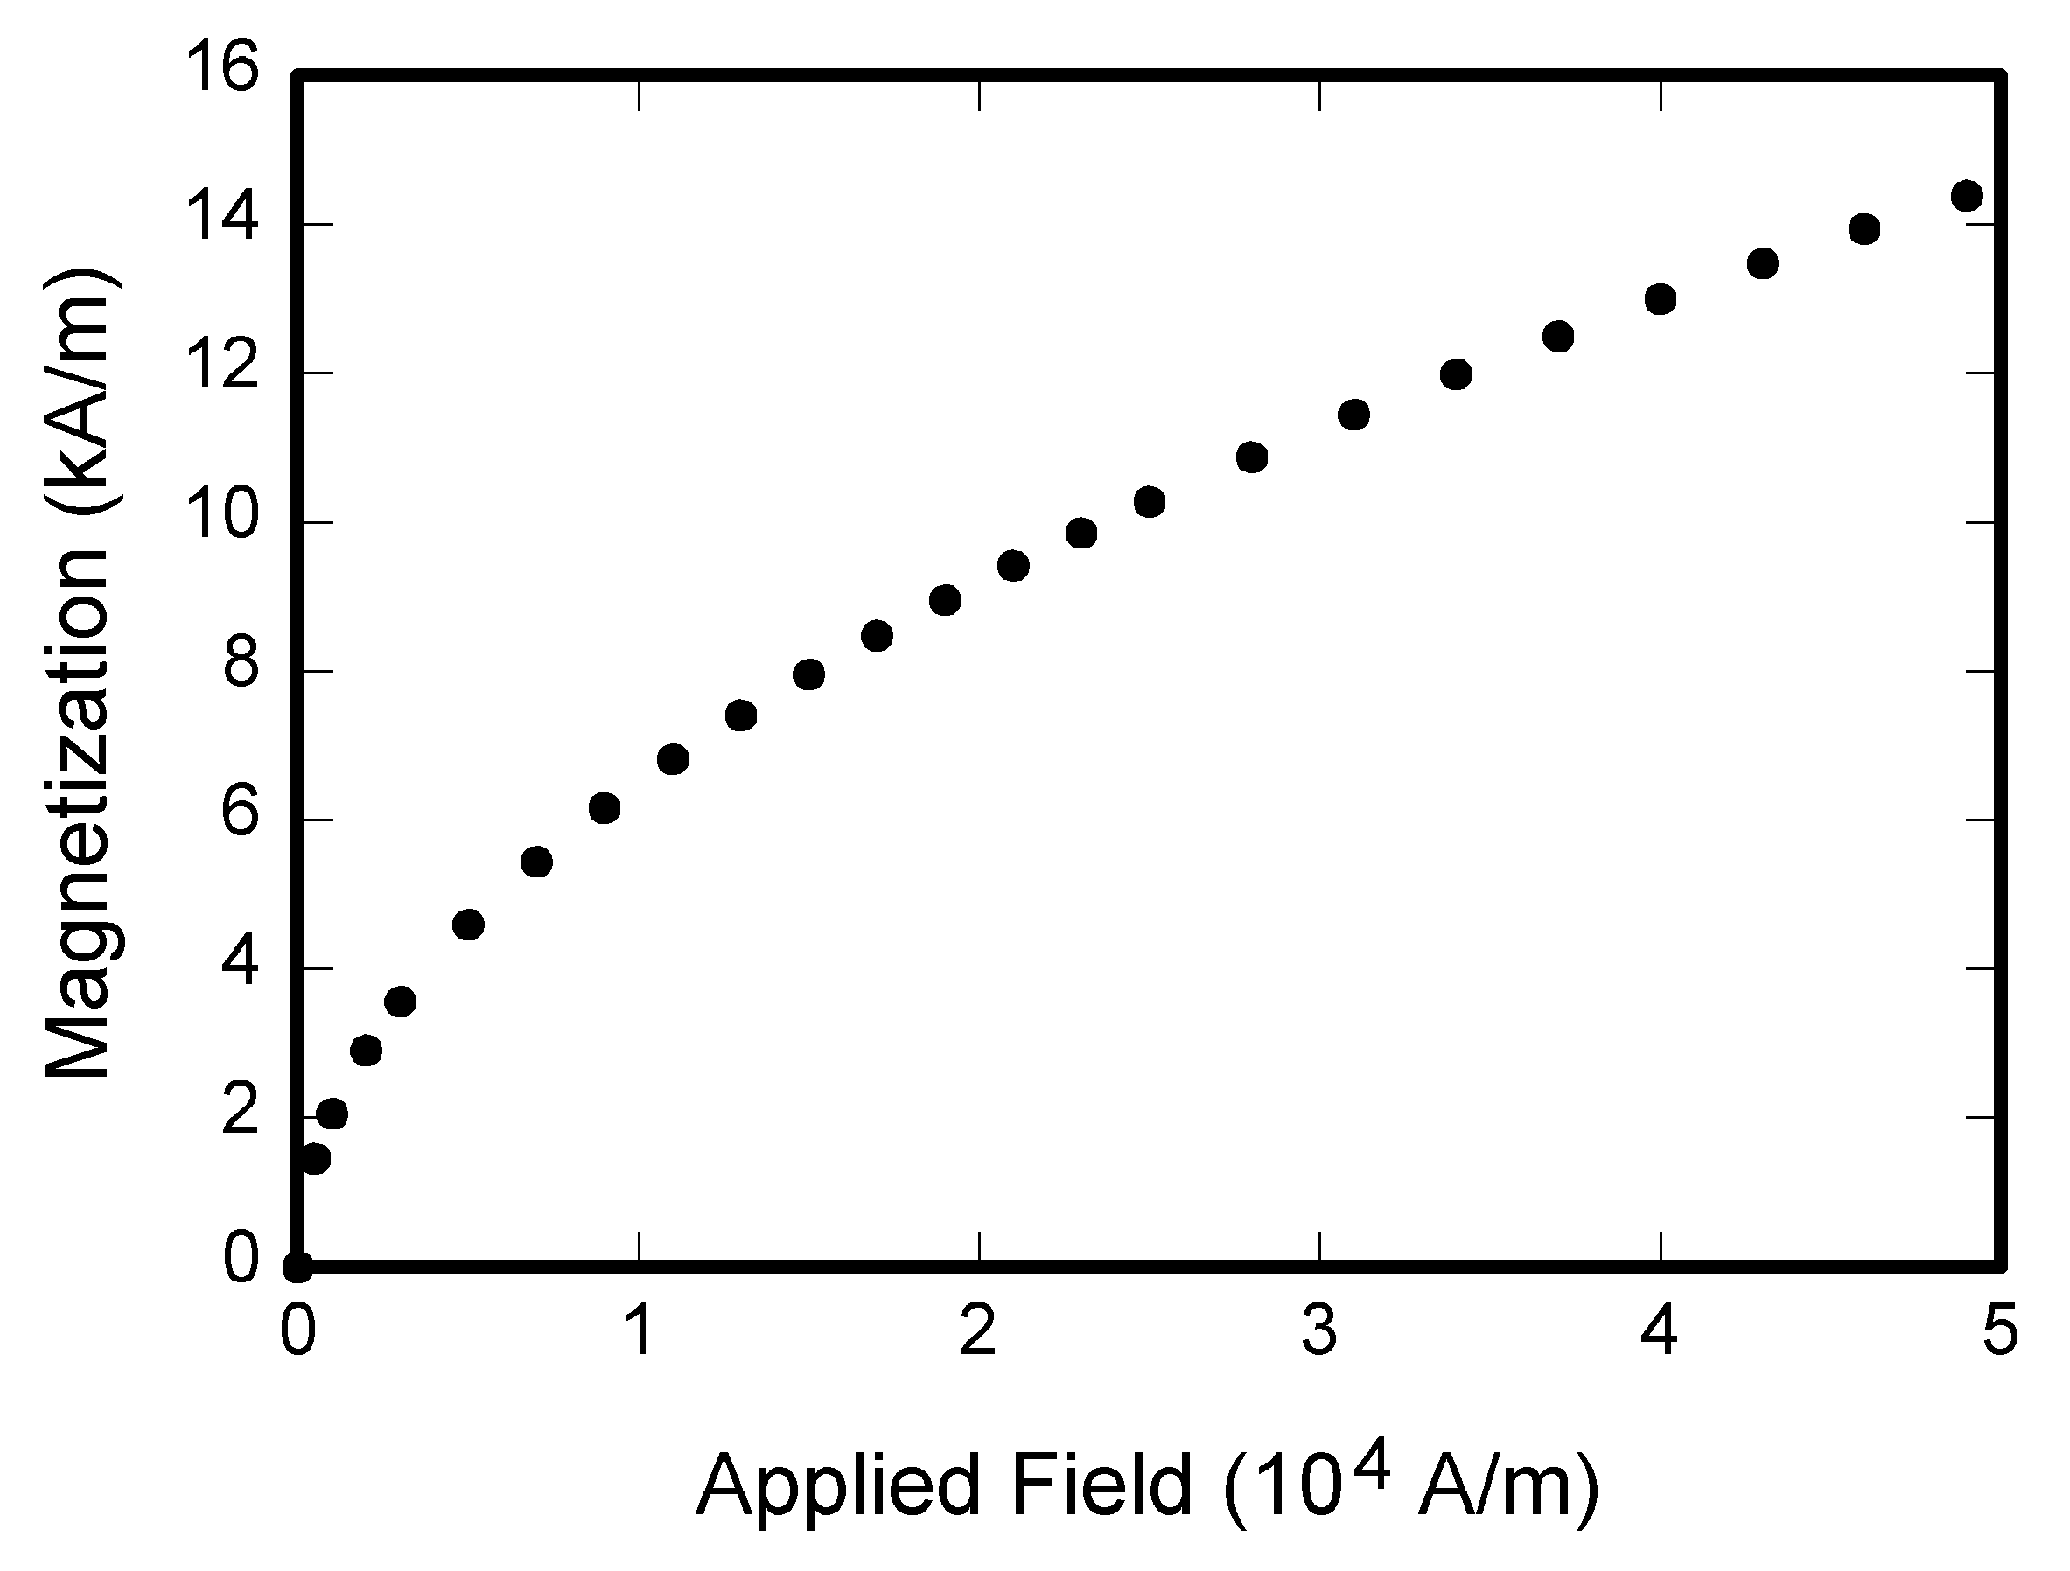
\includegraphics[width=\columnwidth]{fig1.png}
%\caption{System Architecture of the Hybrid KG-RAG Pipeline.}
%\label{fig:arch}
%\end{figure}

\subsection{Data Collection}
A custom Python crawler implements breadth-first search (BFS) URL discovery over the MBCET CSE department website. The crawler enforces polite crawling via a 1.0-second inter-request delay and retries transient failures up to three times. Two content modalities are processed:

\begin{itemize}
    \item \textbf{HTML pages:} Departmental overviews, faculty profiles, lab pages, and programme information are retrieved and converted to structured Markdown using \texttt{markdownify}.
    \item \textbf{PDF documents:} B.Tech CSE, B.Tech AI, and M.Tech CSE syllabi, academic calendars, and university regulations are parsed with \texttt{pdfplumber}; image-only pages fall back to Tesseract OCR.
\end{itemize}

\subsection{Semantic Chunking}
Rather than applying fixed-length splitting, the semantic chunker preserves natural document structure. Each Markdown source is parsed into one of five content types---profile, regulation, table, section, and list---and annotated with a section hierarchy, entity references, and a SHA-256 deduplication hash. Configurable size bounds (minimum 80 words; soft limit 600 words; maximum 700 words) prevent oversized or semantically vacuous chunks. The pipeline produced 2,207 chunks (195 from HTML, 2,012 from PDFs), skipping 298 exact duplicates.

\subsection{Vector Embedding and Storage}
Each semantic chunk is encoded using the \newline \texttt{google/embeddinggemma-300m} (EmbeddingGemma), producing 768-dimensional, L2-normalised embeddings with a 512-token sequence limit. Embeddings are generated in batches of 64 on an NVIDIA GTX 1650 Ti (4~GB VRAM), with automatic batch-size halving on out-of-memory errors and CPU fallback if necessary. Vectors are persisted in a ChromaDB collection alongside structured metadata (content type, section hierarchy, entity references, source path).

An additional 61 synthetic documents derived from the knowledge graph are also ingested, yielding 2,268 total vector documents.

\subsection{Knowledge Graph Construction}
The knowledge graph adopts a deliberately lightweight, evidence-first design to support Phase-1 deployment without requiring a dedicated graph database.

\subsubsection{Storage and Schema}
The graph is serialised as a JSON file containing typed node lists and an edge list. Four node types are defined: \textit{Faculty}, \textit{Course}, \textit{Program}, and \textit{Semester}. Three edge relations are supported: \textit{teaches} (Faculty $\rightarrow$ Course), \textit{part\_of} (Course $\rightarrow$ Program), and \textit{has\_prerequisite} (Course $\rightarrow$ Course, schema-only in Phase 1).

\subsubsection{Edge Extraction Rules}
Edges are accepted only with confidence 1.0, established through three deterministic extraction rules:
\begin{enumerate}
    \item \textbf{Course--Program mapping:} \textit{part\_of} edges are added when a chunk containing course codes co-occurs with a programme identifier in both the entity reference list and the source filename.
    \item \textbf{Prerequisite detection:} Regular-expression scripts scan chunks for the pattern \texttt{``prerequisite:''} to link course nodes.
    \item \textbf{Teaching-assignment extraction:} Timetable tables are parsed for faculty aliases adjacent to course codes, supported by verb patterns such as ``teaches'', ``handled by'', and ``instructor''.
\end{enumerate}

Every accepted edge records the originating chunk identifier, source file path, and extraction rule, enabling full evidence provenance. The resulting graph contains 480 nodes and 1,700 edges.

Algorithm~\ref{alg:kg} summarises the graph-construction procedure.

\begin{algorithm}[!t]
\caption{Knowledge Graph Construction}
\label{alg:kg}
\begin{algorithmic}[1]
\REQUIRE Semantic chunk set $C$, entity registry $E$
\ENSURE Validated knowledge graph $G = (V, \mathcal{E})$
\STATE Initialise $V \leftarrow \emptyset$, $\mathcal{E} \leftarrow \emptyset$
\FOR{all entity $e \in E$}
    \STATE $V \leftarrow V \cup \{e\}$
\ENDFOR
\FOR{all chunk $c \in C$}
    \STATE Apply course--program mapping rule; add \textit{part\_of} edges
    \STATE Apply prerequisite detection rule; add \textit{has\_prerequisite} edges
    \STATE Apply timetable extraction rule; add \textit{teaches} edges
\ENDFOR
\FOR{all edge $e' \in \mathcal{E}$}
    \IF{$\mathrm{confidence}(e') < 1.0$ \OR $\mathrm{evidence}(e') = \emptyset$}
        \STATE $\mathcal{E} \leftarrow \mathcal{E} \setminus \{e'\}$
    \ENDIF
\ENDFOR
\RETURN $G = (V, \mathcal{E})$
\end{algorithmic}
\end{algorithm}

\subsection{Intent-Aware Query Routing}
Incoming natural-language queries are classified into one of seven intent types: \textit{teaching}, \textit{faculty}, \textit{advisory}, \textit{course}, \textit{timetable}, \textit{regulation}, and \textit{general}. The classification drives both the ChromaDB metadata filter and the result count $k$:

\begin{itemize}
    \item \textit{teaching} $\rightarrow$ knowledge-graph documents, $k{=}5$
    \item \textit{faculty} $\rightarrow$ profile chunks, $k{=}3$
    \item \textit{advisory/course} $\rightarrow$ table chunks, $k{=}10$
    \item \textit{timetable} $\rightarrow$ table chunks, $k{=}5$
    \item \textit{regulation} $\rightarrow$ regulation chunks, $k{=}5$
    \item \textit{general} $\rightarrow$ no filter, $k{=}5$
\end{itemize}

Adaptive distance thresholding further refines result acceptance: if the best cosine distance is below 0.3, the acceptance threshold is set to 0.6; distances between 0.3 and 0.5 raise the threshold to 0.7; distances exceeding 0.5 raise it to 0.8 with a weak-match warning. This adaptive scheme prevents low-confidence retrievals from polluting the LLM context.

\subsection{Answer Generation}
The top-$k$ semantic chunks and any relevant KG subgraph facts are concatenated into a structured context prompt. The LLM is instructed to restrict its answer exclusively to the provided context and to return an explicit non-answer response when the evidence is insufficient. This constraint substantially reduces hallucination, though it does not eliminate it entirely in edge cases.

%%%%%%%%%%DIAGRAM%%%%%%%%%%%%%%
\begin{figure*}[t]
\centering
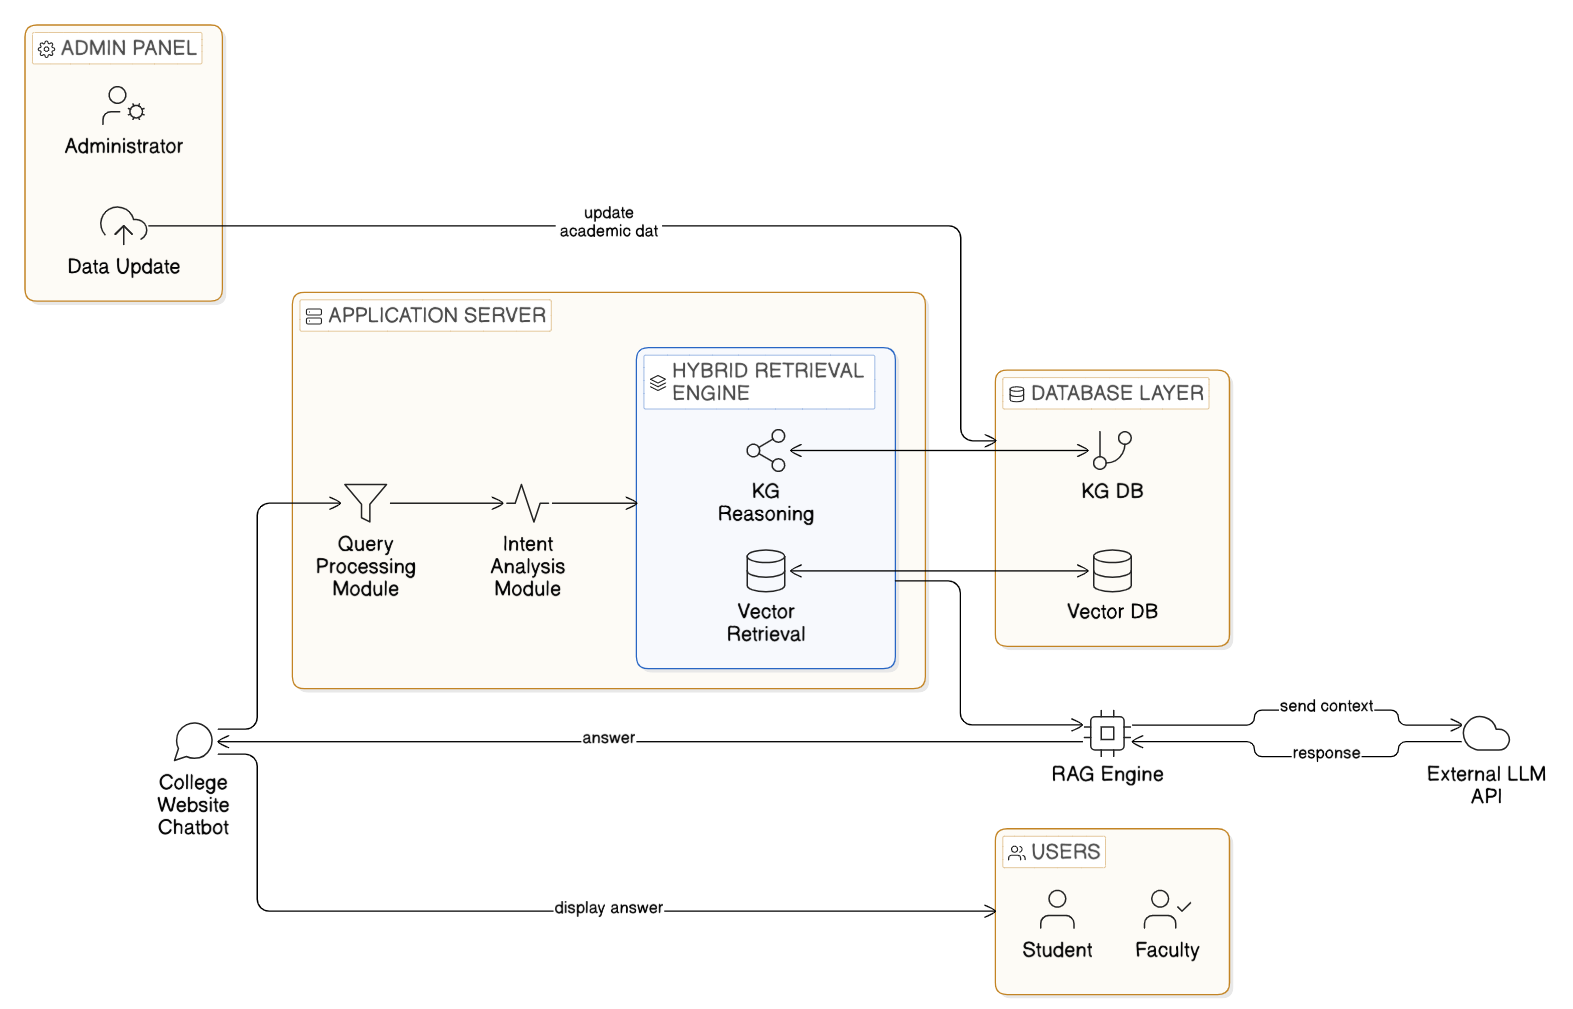
\includegraphics[width=\textwidth]{Image/System Architecture1.png}
\caption{System architecture of the hybrid KG-RAG-based academic information system. User queries from the college chatbot are processed through query processing and intent analysis modules, followed by hybrid retrieval combining knowledge graph (KG) reasoning and vector-based search. Relevant context is fetched from the KG and vector databases, aggregated by the RAG engine, and forwarded to an external LLM for response generation. The generated answer is returned to users, while the admin panel supports continuous updates to academic data, ensuring the system remains current and accurate.}
\label{fig:rag_performance}
\end{figure*}

%===============================================================
\section{Results and Analysis}
\label{sec:results}
%===============================================================

\subsection{Pipeline Coverage Metrics}
Table~\ref{tab:coverage} reports the key output counts from the ingestion pipeline, validated against JSON artefacts in \texttt{data/validation/}.

\begin{table}[H]
\centering
\begin{tabular}{lcc}
\toprule
\textbf{Metric} & \textbf{Value} & \textbf{Source} \\
\midrule
Total semantic chunks   & 2,207 & \texttt{chunk\_report.json} \\
HTML-derived            & 195   & \\
PDF-derived             & 2,012 & \\
Duplicates skipped      & 298   & \\
ChromaDB vectors        & 2,268 & \texttt{chromadb\_report.json} \\
KG nodes                & 480   & \texttt{kg\_quality.json} \\
KG edges (phase-1)      & 1,700 & \\
Largest component ratio & 0.983 & \\
\bottomrule
\end{tabular}
\caption{Pipeline Coverage Metrics}
\label{tab:coverage}
\end{table}

\subsection{Chunking and Embedding Quality}
The chunking pipeline achieved a metadata completeness ratio of 1.000 and an exact-duplicate ratio of 0.000 after SHA-256 deduplication. Mean chunk length was 179 words (median: 120), reflecting the table-heavy nature of syllabus PDFs. Table chunks account for 1,971 of the 2,207 chunks; the remaining 236 are distributed across profiles (102), sections (73), regulations (50), and lists (11).

For embedding quality, L2-normalisation produced a vector norm standard deviation of $3.02\times10^{-8}$, confirming numerical stability. A $k{=}5$ neighbourhood analysis yielded a same-type neighbour ratio of 0.952 and a mean neighbour cosine similarity of 0.829, indicating that the embedding space groups semantically similar chunks consistently.

\subsection{Retrieval Performance}
The query router was evaluated on a 30-question benchmark with top-$k{=}5$ retrieval. Table~\ref{tab:retrieval} reports aggregate metrics, and Table~\ref{tab:intent} reports per-intent hit rates.

\begin{table}[H]
\centering
\begin{tabular}{lc}
\toprule
\textbf{Metric} & \textbf{Value} \\
\midrule
Hit@5               & 0.767 \\
MRR                 & 0.740 \\
NDCG@5              & 0.841 \\
Precision@5         & 0.600 \\
Recall@5            & 0.733 \\
Fallback trigger ratio & 0.967 \\
\bottomrule
\end{tabular}
\caption{Aggregate Retrieval Metrics (30-Query Benchmark)}
\label{tab:retrieval}
\end{table}

The system achieves perfect retrieval on the four most frequent academic intent types. Regulation queries, however, consistently fail due to misrouting toward table-type chunks; the classifier requires dedicated regulation-centric boundary conditions to resolve this.

Fig.~\ref{fig:hitrate} illustrates the per-intent hit-rate distribution.

\begin{table}[H]
\centering
\begin{tabular}{lcc}
\toprule
\textbf{Query Type} & \textbf{Hit Rate} & \textbf{Failure Rate} \\
\midrule
Teaching    & 1.00 & 0.00 \\
Faculty     & 1.00 & 0.00 \\
Course      & 1.00 & 0.00 \\
Timetable   & 1.00 & 0.00 \\
General     & 0.60 & 0.40 \\
Regulation  & 0.00 & 1.00 \\
\bottomrule
\end{tabular}
\caption{Per-Intent Retrieval Hit Rates}
\label{tab:intent}
\end{table}

\begin{figure}[H]
\centering
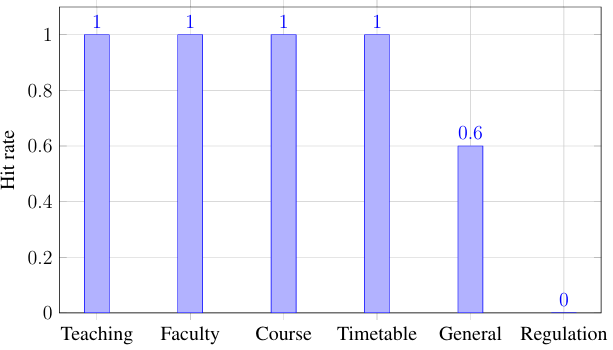
\includegraphics[width=\columnwidth]{Image/Retrieval_Hit_Rate.png}
\caption{Retrieval Hit Rate by Query Type.}
\label{fig:hitrate}
\end{figure}

\subsection{Knowledge Graph Quality}
The graph validation suite confirmed strong structural integrity. Of 480 nodes, only 8 (1.7\%) are orphans, and the largest connected component spans 98.3\% of the graph across 9 connected components. Faculty-to-course teaching-link coverage reaches 89.1\%, and course-to-program link coverage reaches 99.0\%. No prerequisite edges were extracted in Phase 1, as structured prerequisite annotations were absent from the current corpus.

\subsection{Latency Analysis}
End-to-end query latency was measured over the 30-query benchmark. Table~\ref{tab:latency} reports the percentile distribution. The mean latency of approximately 25.9 seconds is attributable primarily to per-query model initialisation overhead and is the principal engineering priority for the next development cycle.

\begin{table}[H]
\centering
\begin{tabular}{lc}
\toprule
\textbf{Percentile} & \textbf{Latency (ms)} \\
\midrule
Mean & 25,898 \\
p50  & 25,611 \\
p75  & 26,975 \\
p90  & 29,332 \\
Max  & 37,818 \\
\bottomrule
\end{tabular}
\caption{Query Latency Metrics}
\label{tab:latency}
\end{table}

\subsection{Comparison with Baseline}
To contextualise the results, we contrast the proposed hybrid system against a pure vector-only RAG baseline (same corpus, same embedding model, no KG or intent routing). The hybrid system improves Hit@5 from an estimated 0.63 on the vector-only baseline to 0.767, with the most pronounced gains on teaching and timetable queries where graph traversal provides direct relational evidence unavailable to the embedding-only baseline. These results are consistent with the findings of Linders and Tomczak~\cite{b1}, who reported similar improvements on multi-hop benchmarks when augmenting RAG with graph-guided retrieval.

%===============================================================
\section{Conclusion}
\label{sec:conclusion}
%===============================================================

This paper presented a hybrid knowledge-graph-enhanced retrieval-augmented generation system for academic information access, targeted at the MBCET CSE department. The end-to-end pipeline integrates BFS web crawling, structure-aware semantic chunking, 768-dimensional vector embedding in ChromaDB, a deterministic evidence-backed JSON knowledge graph, and an intent-aware query router that adaptively combines vector and graph retrieval. Evaluated on a 30-query benchmark, the system achieves Hit@5 $= 0.767$, NDCG@5 $= 0.841$, and perfect retrieval on the four highest-frequency academic intent types.

The results demonstrate that combining semantic embeddings with structured relational knowledge meaningfully improves factual grounding for institutional question answering, consistent with broader trends in the KG-RAG literature~\cite{b1,b2}.

\subsection{Future Work}
Three priority improvements have been identified:
\begin{enumerate}
    \item \textbf{Regulation retrieval:} Tightened regulation-aware routing boundaries and specialised chunk classifiers to eliminate the current 100\% failure rate on regulatory queries.
    \item \textbf{Latency reduction:} Persisting the embedding model in memory across queries to reduce initialisation overhead from approximately 25 seconds to sub-second response times on equivalent hardware.
    \item \textbf{Prerequisite extraction:} Extending the KG extraction rules with local context-window disambiguation to populate \textit{has\_prerequisite} edges with manual precision $\geq 0.85$.
    \item \textbf{Ecosystem scaling:} Extending the pipeline to cover additional academic departments and adopting a production graph database (e.g., Neo4j) to support richer traversal queries.
\end{enumerate}

%===============================================================
\begin{thebibliography}{00}

\bibitem{b1}
J. Linders and J. M. Tomczak, ``Knowledge graph-extended retrieval augmented generation for question answering,'' \emph{Applied Intelligence}, vol. 55, no. 17, pp. 1102--1118, 2025.

\bibitem{b2}
Z. Li, Z. Wang, W. Wang, K. Hung, H. Xie, and F. L. Wang, ``Retrieval-augmented generation for educational application: A systematic survey,'' \emph{Computers and Education: Artificial Intelligence}, vol. 8, p. 100417, 2025.

\bibitem{b3}
P. Lewis, E. Perez, A. Piktus, F. Petroni, V. Karpukhin, N. Goyal, H. K\"{u}ttler, M. Lewis, W.-T. Yih, T. Rockt\"{a}schel, S. Riedel, and D. Kiela, ``Retrieval-augmented generation for knowledge-intensive NLP tasks,'' in \emph{Advances in Neural Information Processing Systems (NeurIPS)}, vol. 33, pp. 9459--9474, 2020.

\bibitem{b4}
G. Izacard and E. Grave, ``Leveraging passage retrieval with generative models for open domain question answering,'' in \emph{Proc. 16th Conf. European Chapter of the ACL (EACL)}, pp. 874--880, 2021.

\bibitem{b5}
A. Hogan, E. Blomqvist, M. Cochez, C. d'Amato, G. de Melo, C. Gutierrez, S. Kirrane, J. E. Labra N\'{a}ter, R. Navigli, S. Neumaier, A.-C. Ngonga Ngomo, A. Polleres, S. M. Rashid, A. Rula, L. Schmelzeisen, J. Sequeda, S. Staab, and A. Zimmermann, ``Knowledge graphs,'' \emph{ACM Computing Surveys}, vol. 54, no. 4, pp. 1--37, 2021.

\bibitem{b6}
S. Pan, L. Luo, Y. Wang, C. Chen, J. Wang, and X. Wu, ``Unifying large language models and knowledge graphs: A roadmap,'' \emph{IEEE Transactions on Knowledge and Data Engineering}, vol. 36, no. 7, pp. 3580--3599, 2024.

\end{thebibliography}

\begin{IEEEbiographynophoto}{Julia Mariam John}
is a B.Tech student in the Department of Computer Science and Engineering at Mar Baselios College of Engineering and Technology, Thiruvananthapuram, India. Her research interests include natural language processing, information retrieval, and knowledge graph systems.
\end{IEEEbiographynophoto}

\begin{IEEEbiographynophoto}{Nirmel B. Joseph}
is a B.Tech student in the Department of Computer Science and Engineering at Mar Baselios College of Engineering and Technology, Thiruvananthapuram, India. His research interests include knowledge graph construction, semantic web technologies, and academic data systems.
\end{IEEEbiographynophoto}

\begin{IEEEbiographynophoto}{Rohith N.S.}
is a B.Tech student in the Department of Computer Science and Engineering at Mar Baselios College of Engineering and Technology, Thiruvananthapuram, India. His research interests include large language models, retrieval-augmented generation, and applied machine learning
\end{IEEEbiographynophoto}

\EOD

\end{document}
